%!TEX root = proposta.tex 
\chapter{\label{chap:descr}Descrição do Projeto}

\section{Algoritmo}
O algoritmo a ser implementado é o AHTN. Nele são combinados tecnicas de HTN com o algoritmo \textit{minimax game tree search}\frm{Algoritmo o qual tu não falou nada ainda!! Aqui tu deixa muita coisa picando!}. 
%algoritmo a ser utilizado \\
%algoritmo de ML a ser agregado

\section{Ambiente}

%\frm[inline]{Remover os passivos}
%O ambiente que será utilizado é o MicroRTS. 
Utilizaremos o jogo MicroRTS como plataforma de teste para o algoritmo AHTN. O jogo MicroRTS foi feito por Santiago Ontañón \cite{ontanon2013combinatorial} para fins acadêmicos, com o intuito de aplicar e desenvolver técnicas de IA e para servir como prova de conceito para as técnicas criadas.  
O jogo é uma simplificação do jogo Starcraft\footnote{http://us.battle.net/sc2/pt/}. O jogo é um jogo RTS contra um adversário. O objetivo do jogo é destruir a base adversaria. Existem trabalhadores que podem coletar recursos e construir outros prédios. Os recursos são coletados dos minerais. Com os recursos é possivel construir bases de ataque, onde são realizado o treinamento de unidades de ataque. Para conseguir realizar o objetivo de destruir a base adversaria é preciso ter unidades de ataque. O jogo oferece três destas unidades, são elas:

\begin{itemize}
	\item Heavy - Possui um alto poder de ataque, mas sua velocidade é lenta.
	\item Light - Possui um baixo poder de ataque, mas sua velocidade é rapida.
	\item Ranged - Possui um ataque de longa distancia. 
\end{itemize} 

A Figura~\ref{fig:microrts}\footnote{https://github.com/santiontanon/microrts} mostra uma tela do jogo que representa o que foi explicado. É possível observar que o fator de ramificação pode ser muito alto dependendo do cenário do jogo. %\frm{Figura sem explicação... Só os comentários do lado, em inglês, não te resolvem}

\begin{figure}[ht]
	\centering
	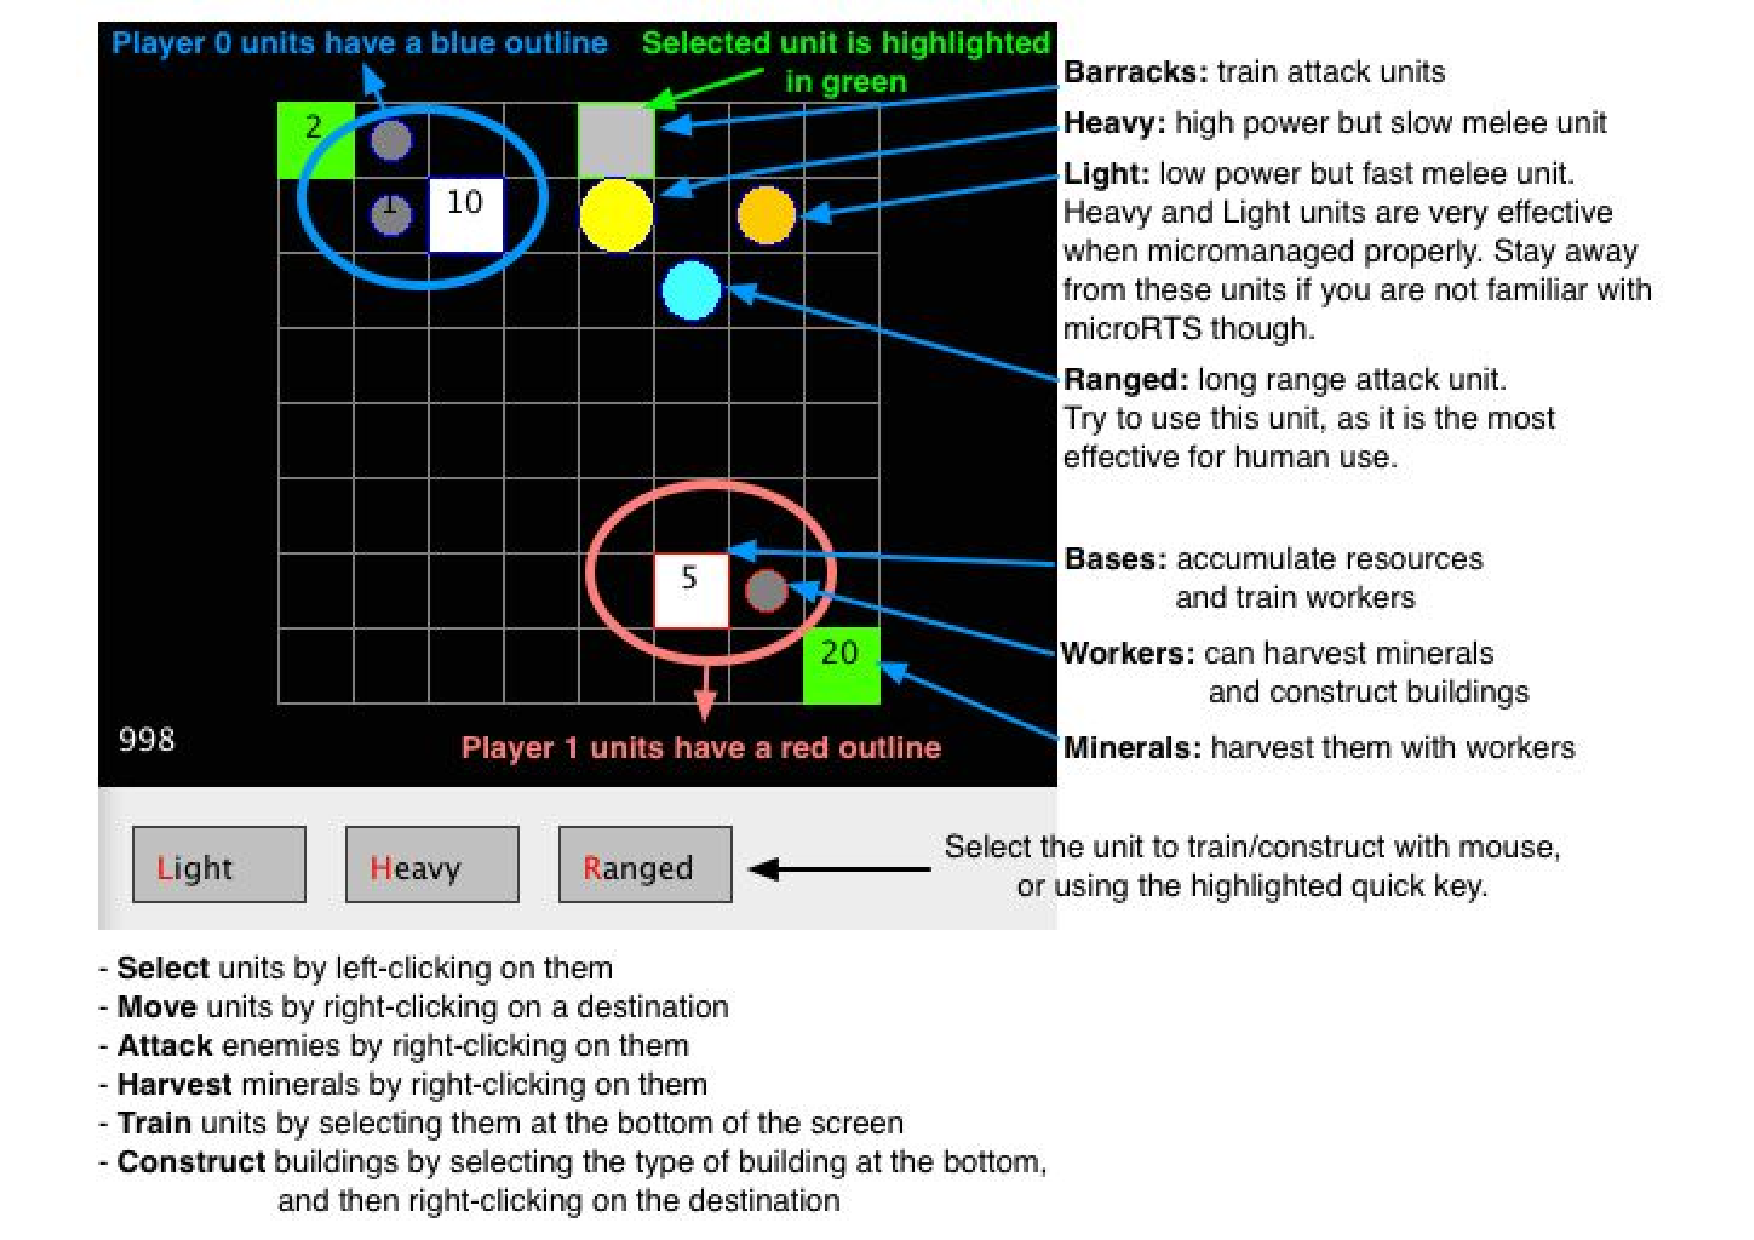
\includegraphics[width=0.8\textwidth]{fig/microrts.pdf}
	\caption{Uma foto da tela do MicroRTS}
	\label{fig:microrts}
\end{figure} 

No ambiente há algumas estrategias implementadas, cada estrategia possui variações dos algoritmos. Algumas das estrategias são:
\begin{itemize}
	\item Minimax Alpha-Beta Search Strategies - O que muda entre as técnicas é o jeito com que é feito a expansão do grafo.
	\item Monte Carlo Search Strategies - Executa jogadas aleatórias para planejar e após utiliza uma heurística para determinar em qual caminho seguir.
\end{itemize}

%\frm[inline]{E.. depois da itemização talvez seja interessante concluir algo}
A plataforma já foi utilizada para aplicar técnica de IA. Por esse motivo a utilização desta plataforma se torna viável. A comparação entre as estrategias já existentes com a que estou propondo pode mostrar que a
 abordagem resulta em um melhor desempenho. 
